\hypertarget{oppgave2}{}
\section*{Oppgave 2}
\addcontentsline{toc}{section}{Oppgave 2}
% ==================================================
% OPPGAVE 2
% ==================================================

% --------------------------------------------------
\subsection*{a)}
Fra det gitte linjespekteret kan de komplekse frekvenskomponentene leses av som:
\[
\begin{array}{c|c}
f\,[\mathrm{Hz}] & C_f \\ \hline
-250 & 4e^{-j\pi/2} \\
-100 & 7e^{j\pi/3} \\
0    & 10 \\
100  & 7e^{-j\pi/3} \\
250  & 4e^{j\pi/2}
\end{array}
\]
Magnitudespekteret finnes ved å ta absoluttverdien av de komplekse koeffisientene:
\[
\begin{array}{c|c}
f\,[\mathrm{Hz}] & |C_f| \\ \hline
-250 & 4 \\
-100 & 7 \\
0    & 10 \\
100  & 7 \\
250  & 4
\end{array}
\]
Fasespekteret finnes fra vinkelen til de komplekse koeffisientene:
\[
\begin{array}{c|c}
f\,[\mathrm{Hz}] & \angle C_f \\ \hline
-250 & -\pi/2 \\
-100 & \pi/3 \\
0    & 0 \\
100  & -\pi/3 \\
250  & \pi/2
\end{array}
\]
Magnitudespekteret er symmetrisk rundt $f=0$, mens fasen har motsatt fortegn for positive og negative frekvenser.
\begin{figure}[H]
    \centering
    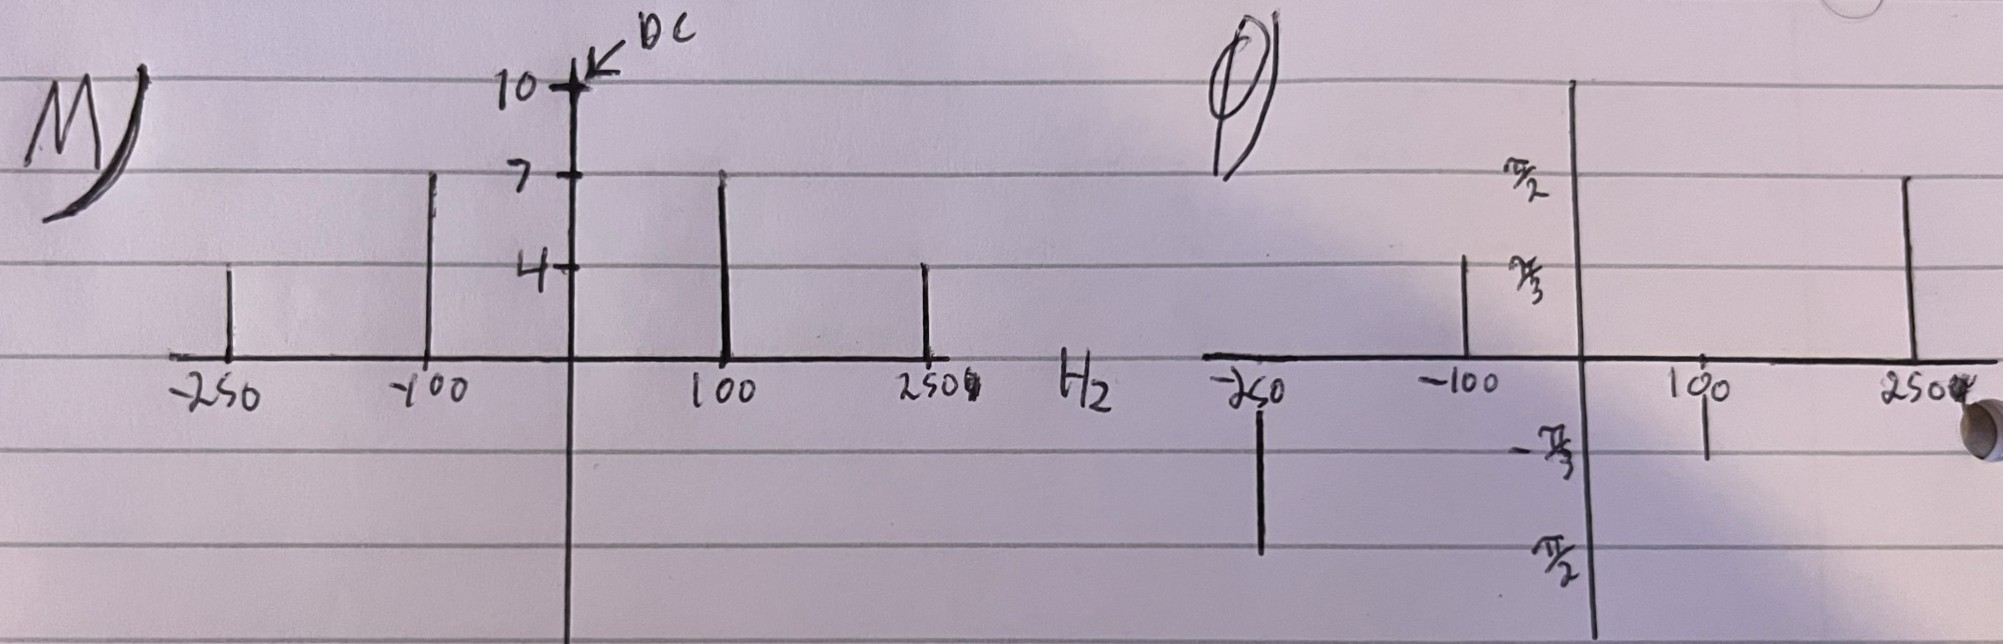
\includegraphics[width=1\textwidth]{Media/bg.jpg}
    \caption{Magnitudespekteret og fasespekteret til signalet $s(t)$.}
    \label{fig:oppgave2a}
\end{figure}
% --------------------------------------------------
\subsection*{b)}
Signalet inneholder frekvenskomponenter ved 100 Hz og 250 Hz.
Begge frekvensene kan skrives som heltallsmultipler av en felles grunnfrekvens:
\[
    \mathrm{gcd}(100, 250) = 50 \text{ Hz}.
\]
Grunnfrekvensen blir derfor:
\[
f_0=50\text{ Hz}.
\]
Signalet er periodisk fordi alle frekvenskomponentene er heltallsmultipler av den samme grunnfrekvensen $f_0$.
Periodetiden blir:
\[
T_0=\frac{1}{f_0}
=\frac{1}{50}
=0.02\text{ s}.
\]
Dermed er:
\[
\boxed{T_0=20\text{ ms}}.
\]
% --------------------------------------------------
\subsection*{c)}
De komplekse frekvenskomponentene ved positiv og negativ frekvens kan kombineres til cosinusledd.
Ved $f=100$ Hz har hver frekvenskomponent magnitude 7.
Amplituden til cosinusleddet blir derfor:
\[
A=2\cdot7=14.
\]
Fasen ved den positive frekvensen er $-\pi/3$, som gir:
\[
14\cos\left(2\pi100t-\frac{\pi}{3}\right).
\]
Ved $f=250$ Hz har hver frekvenskomponent magnitude 4.
Amplituden til cosinusleddet blir derfor:
\[
A=2\cdot4=8.
\]
Fasen ved den positive frekvensen er $\pi/2$, som gir:
\[
8\cos\left(2\pi250t+\frac{\pi}{2}\right).
\]
I tillegg inneholder signalet en DC-komponent på 10.
Signalet kan derfor skrives som:
\[
\boxed{
s(t)=10
+14\cos\left(2\pi100t-\frac{\pi}{3}\right)
+8\cos\left(2\pi250t+\frac{\pi}{2}\right)
}.
\]